% -*- root: ../Presentation.tex -*-
\section{Hiding Data in JPEG Images}
%PNG SECTION
\begin{frame}{Hiding Data in JPEG Images}{}
	\begin{minipage}[0.5\textheight]{\textwidth}
		\begin{columns}[T]
			\begin{column}{0.5\textwidth}
				\begin{itemize}
					\item In PNG images all pixels can be changed separately
					\item Enables the use of methods such as LSB with a very high payload
				\end{itemize}
			\end{column}
			\begin{column}{0.5\textwidth}
				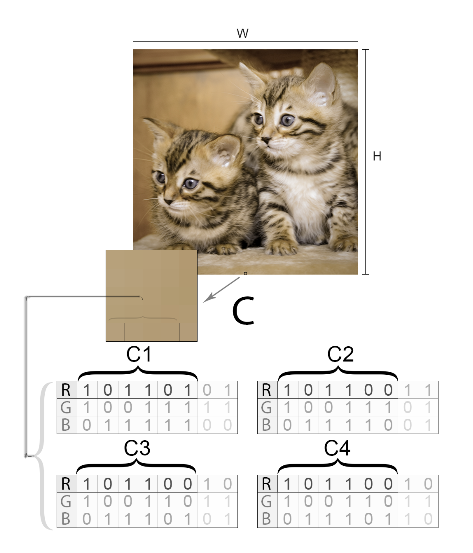
\includegraphics[width=\textwidth]{figures/pngImage.png}
			\end{column}
		\end{columns}
	\end{minipage}
\end{frame}
%JPEG SECTION
\begin{frame}{Hiding Data in JPEG Images}{}
	\begin{minipage}[0.5\textheight]{\textwidth}
		\begin{columns}[T]
			\begin{column}{0.5\textwidth}
				\vspace{.56mm}
				\begin{itemize}
					\item JPEG images are divided into MCUs
					\item Further divided into 8x8 blocks
					\item After performing DCT and quantization there is an 8x8 block of integers
				\end{itemize}
			\end{column}
			\begin{column}{0.5\textwidth}
				\begin{center}
					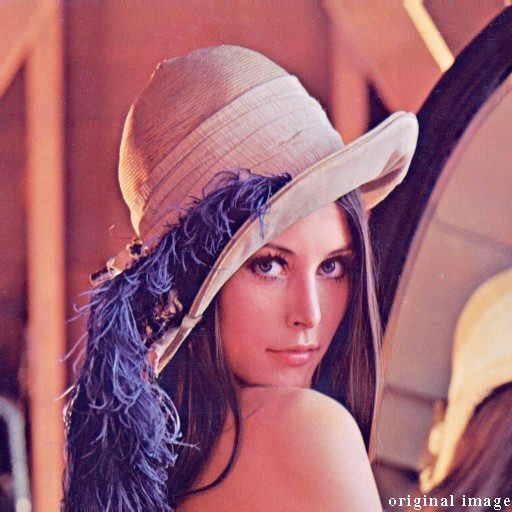
\includegraphics[width=.5\textwidth]{figures/lena_color.jpg}
				\end{center}
				{\tiny \begin{table}[]
				\centering
					\begin{tabular}{|c|c|c|c|c|c|c|c|}
					\hline
					-26 & -3 & -6 & 2  & 2  & -1 & 0 & 0 \\ \hline
					0   & -2 & -4 & 1  & 1  & 0  & 0 & 0 \\ \hline
					-3  & 1  & 5  & -1 & -1 & 0  & 0 & 0 \\ \hline
					-3  & 1  & 2  & -1 & 0  & 0  & 0 & 0 \\ \hline
					0   & 0  & 0  & 0  & 0  & 0  & 0 & 0 \\ \hline
					0   & 0  & 0  & 0  & 0  & 0  & 0 & 0 \\ \hline
					0   & 0  & 0  & 0  & 0  & 0  & 0 & 0 \\ \hline
					0   & 0  & 0  & 0  & 0  & 0  & 0 & 0 \\ \hline
					\end{tabular}
				\end{table}
				}
			\end{column}
		\end{columns}
	\end{minipage}
\end{frame}


\subsection{Techniques}
\begin{frame}{Techniques of Hiding Data in JPEG Images}{}
	\begin{itemize}
		\item<1 -> A naive approach to hiding data is simply appending the clear text to the image
		\item<2 -> A better approach is to trick the decoder with APP$_n$ segments
		\item<3 -> Maybe try to use the LSB method on DCT tables?
		\begin{itemize}\item<4 -> On thumbnail?\end{itemize}
		\item<5 -> A Graph-theoretic approach
	\end{itemize}
\end{frame}
